\documentclass[11pt]{extarticle}
\usepackage[T1]{fontenc}
\usepackage{amsmath}
\usepackage{amsthm}
\usepackage{amsfonts}
\usepackage{amssymb}
\usepackage{xcolor}	
\usepackage{graphicx}
\usepackage{caption}
\usepackage{subcaption}
\usepackage{multirow}
\usepackage{float}
\usepackage{enumitem}
\usepackage{titlesec}
%\usepackage{hyperref}

\usepackage{pdflscape}
\usepackage{fancyhdr}
\usepackage{booktabs}

% Show line numbers
\usepackage[mathlines]{lineno}
\renewcommand\linenumberfont{\normalfont\small\color{gray}}
% \linenumbers

% Show labels
% \usepackage{showlabels}

\newsavebox{\dnbox}
\newsavebox{\dntab}

% Float placement: the defaults are too restrictive for the large
% figure/table pairs of Section 4 and push them onto pages of their own.
\renewcommand{\topfraction}{0.9}
\renewcommand{\bottomfraction}{0.8}
\renewcommand{\textfraction}{0.07}
\renewcommand{\floatpagefraction}{0.8}

\numberwithin{equation}{section}
\usepackage{lipsum}
\setlength{\textwidth}     {16.0cm}
\setlength{\textheight}    {21.0cm}
\setlength{\evensidemargin}{ 0.0cm}
\setlength{\oddsidemargin} { 0.0cm}
\setlength{\topmargin}     {-0.5cm}
\setlength{\baselineskip}  { 0.7cm}


\newcommand{\R}{\mathbb{R}}
\newcommand{\D}{\mathbb{D}}
\newcommand{\C}{\mathbb{C}}
\newcommand{\N}{\mathbb{N}}
\newcommand{\Z}{\mathbb{Z}}
\newcommand{\dirichlet}{\mathcal{H}^2}

\theoremstyle{plain}
\newtheorem{example}{Example}[section]
\newtheorem{theorem}{Theorem}[section]
\newtheorem{corollary}{Corollary}[section]
\newtheorem{lemma}{Lemma}[section]
\newtheorem{proposition}{Proposition}[section]
\newtheorem{axiom}{Axiom}[section]
\newtheorem{remark}{Remark}[section]
\theoremstyle{definition}
\newtheorem{definition}{Definition}[section]
\newtheorem{assumption}{Assumption}
\renewcommand\theassumption{A\arabic{assumption}}
\newcommand{\expnumber}[2]{{#1}\mathrm{E}{#2}}


\begin{document}

\title{A Hardy space approximation supporting zero-free half-planes for the $\zeta$-function}

\author{
    Juan Manzur\thanks{Department of Mathematics,
    Universidad del Atlántico, Puerto Colombia, Atlántico, Colombia. email: jcmanzur@mail.uniatlantico.edu.co}
    \and
    Gustavo Quintero\thanks{Department of Mathematics, Universidad del Atlántico, Puerto Colombia, Atlántico, Colombia. email: gdquintero@mail.uniatlantico.edu.co}
}

\date\today
\maketitle

\begin{abstract}

 Bagchi's Hilbert-space reformulation of the Báez-Duarte criterion \cite{baez} for the Riemann Hypothesis (RH) \cite{bagchi} states that RH holds if and only if $E(s)=1/s$ belongs to the closed linear span of $\{G_k : k\geq 2\}$, where $G_k(s)=(k^{-s}-k^{-1})\zeta(s)/s$, in the Hardy space $H^2(\C_{1/2})$; here $\C_\alpha$ denotes the half-plane $\mathrm{Re}(s)>\alpha$. We prove that $\sum_{k=2}^{\infty}\mu(k)G_k$ converges to $E$ in $H^2(\C_\alpha)$ for every $\alpha>1$; together with the fact that membership of $E$ in the span forces $\zeta$ to be zero-free in $\C_\alpha$, this gives an approximation-theoretic route recovering the classical non-vanishing of $\zeta$ on
$\mathrm{Re}(s)>1$. A matching quantitative result shows that $\alpha_c := \inf\{\alpha\geq1/2 : d_n(\alpha)^2\to0\}$, the threshold at which the best $n$-term approximation of $E$ converges, equals $1/2$ if and only if RH holds. Motivated by this equivalence, we numerically study the Möbius error $s_n(\alpha) = \|\sum_{k=2}^n\mu(k)G_k - E\|^2_\alpha$ for $1/2\leq\alpha\leq1$, where $\|\cdot\|_\alpha$ denotes the norm of $H^2(\C_\alpha)$, and the optimal error $d_n(1/2)^2$ on the critical line. An exact formula expressing $s_n(\alpha)$ as a series with elementary terms, free of the zeta function, allows us to compute it up to $n = 10^6$: on the critical line $s_n(1/2)$ oscillates without decaying, consistent with its known divergence, while for every $\alpha > 1/2$ the oscillations decay at a rate close to $n^{1-2\alpha}$.

\bigskip
\noindent
\textbf{Keywords:} Riemann hypothesis, zero-free half-planes, B\'aez-Duarte criterion, Hardy spaces, numerical approximation.
% \textbf{Keywords:} Riemann hypothesis, simulations, Nymann-Beurling.\\

% \noindent
% \textbf{Mathematics Subject Classification:} 90C30, 65K05, 49M37, 90C60, 68Q25.\\
\end{abstract}



\section{Introduction}

The Riemann Hypothesis (RH) asserts that all non-trivial zeros of the Riemann 
zeta function lie on the critical line $\mathrm{Re}(s) = \frac{1}{2}$. Its 
implications for the distribution of prime numbers make it one of the central 
open problems in mathematics.

A functional-analytic approach to RH was initiated by Nyman and Beurling, who 
showed that RH is equivalent to the density of a specific family of functions 
in $L^2(0,1)$~\cite{beurling,Nyman}. Báez-Duarte later refined this by 
replacing the original uncountable family with a countable sequence, simplifying 
the problem while preserving its essential structure~\cite{baez}. Balazard and
Saias~\cite{Balazard} extended this approach to a weighted $\ell^2$-sequence space by posing the question of whether the orthogonal projection coefficients $c_{n,k}$ of $\mathbf{1}$ onto $\mathrm{span}\{r_k : 
2 \leq k \leq n\}$ satisfy
\[
\lim_{n\to\infty} c_{n,k} = -\frac{\mu(k)}{k}, \quad \forall\, k \geq 2,
\]
where $\mu$ is the Möbius function and $r_k(j) = j \bmod k$ denotes the 
remainder upon division of $j$ by $k$. This condition was shown by Weingartner in \cite{Weingartner} 
to be equivalent to the RH, which identifies $-\mu(k)/k$ as the natural, and in a precise sense optimal, choice of coefficients.

A reformulation within the Hardy space $H^2(\mathbb{C}_{1/2})$ was established 
by Bagchi~\cite{bagchi}, where $\mathbb{C}_\alpha = \{s \in \mathbb{C} : \mathrm{Re}(s) > \alpha\}$ 
for $\alpha \in \mathbb{R}$: RH holds if and only if $E(s) = 1/s$ belongs to the 
closed linear span of
\[
G_k(s) = \bigl(k^{-s} - k^{-1}\bigr)\frac{\zeta(s)}{s}, \quad k \geq 2,
\]
in $H^2(\mathbb{C}_{1/2})$. Building on these ideas, Noor introduced an 
equivalent reformulation in the Hardy--Hilbert space $H^2(\mathbb{D})$ of the 
unit disk~\cite{waleed1}: RH holds if and only if the constant function 
$\mathbf{1}$ belongs to the closed linear span of
\[
h_k(z) = \frac{1}{1-z}\log\!\left(\frac{1+z+\cdots+z^{k-1}}{k}\right), \quad k \geq 2.
\]
In the same work, Noor established that the series $\sum_{k=2}^{\infty} 
\frac{\mu(k)}{k}(I-S)h_k$ converges to $1-z$ in $H^2(\mathbb{D})$, where 
$S$ is the shift operator. For an overview of the various equivalent reformulations of the Nyman-Beurling and Báez-Duarte approaches that appear in the literature, see \cite[p. 5-6]{noor-charles}.

The main idea of this paper is to generalize this 
result in an attempt to approximate RH using the reformulation of Bagchi in 
$H^2(\mathbb{C}_{1/2})$. To achieve this, we employ the Hilbert space of 
Dirichlet series $\mathcal{H}^2$, which is naturally connected to 
the Hardy space of the disk. Within this framework, we construct a bounded 
operator $\mathcal{M}^\tau$ that establishes a connection between $\mathcal{H}^2$ 
and the Hardy spaces $H^2(\mathbb{C}_\alpha)$, leading to our main result 
(Theorem~\ref{main-teo}): the series $\sum_{k=2}^{\infty}\mu(k)G_k$ converges 
to $E$ in $H^2(\mathbb{C}_\alpha)$ for every $\alpha > 1$. Furthermore, 
Proposition~\ref{main-prop} establishes that for any $\alpha \geq 1/2$,
\[
E \in \overline{\mathrm{span}}\{G_k : k \geq 2\} \ \text{in }
H^2(\mathbb{C}_\alpha) \implies \zeta(s) \neq 0, \quad \forall\, s \in \mathbb{C}_\alpha.
\]

A quantitative counterpart also holds. For $n \geq 2$ and $\alpha > 0$, let
\[
d_n(\alpha)^2 := \inf_{c_2, \dots, c_n \in \mathbb{C}} \Bigl\| E - \sum_{k=2}^{n} c_k G_k \Bigr\|^2_\alpha
\]
denote the optimal approximation error over all coefficients. Theorem~\ref{thm:lower} shows that a
single zero of $\zeta$ in $\mathbb{C}_\alpha$ forces $d_n(\alpha)^2$ to stay
bounded away from $0$, uniformly in $n$. Combined with
Proposition~\ref{main-prop}, this yields Corollary~\ref{cor:sensor}: writing
$\Theta$ for the supremum of the real parts of the zeros of $\zeta$ and
$\alpha_c = \inf\{\alpha \geq 1/2 : d_n(\alpha)^2 \to 0\}$, one has
$1/2 \leq \Theta \leq \alpha_c \leq 1$, with $\alpha_c = 1/2$ if and only if RH
holds. This recasts RH as a statement about the asymptotic behaviour of
$d_n(\alpha)^2$, and is what motivates the numerical study of $d_n(1/2)^2$ in
Subsection~\ref{subsec:dn}.

An important question that arises is whether the convergence of the series
extends to $1/2 \leq \alpha \leq 1$. Báez-Duarte~\cite{baez-unitary} showed
that the $L^2(0,1)$-analog of the sequence $s_n(\alpha)$ defined below diverges, which implies the divergence of $s_n(1/2)$ itself
in $H^2(\mathbb{C}_{1/2})$. Studying the convergence in the range
$1/2 < \alpha \leq 1$ is therefore essential, as it could provide information
about zero-free regions of $\zeta$ within the critical strip, a notoriously
hard problem in its own right.

The numerical analysis conducted in this work addresses two questions. The
first is whether the convergence of the partial sums
\[
s_n(\alpha) = \left\|\sum_{k=2}^{n}\mu(k)G_k - E\right\|^2_\alpha
\]
persists beyond the range $\alpha > 1$ settled by Theorem~\ref{main-teo}. To study
it we express $s_n(\alpha)$ exactly as a series with elementary terms
(Proposition~\ref{prop:exact}), which avoids both the zeta function and numerical
quadrature and allows us to compute $s_n(\alpha)$ up to $n = 10^6$ for
$1/2 \leq \alpha \leq 1$. On the critical line $s_n(1/2)$ oscillates without
decaying, consistent with the divergence result of Báez-Duarte, whereas for every
$\alpha > 1/2$ the oscillations decay, at a rate close to $n^{1-2\alpha}$.
The second question, guided by Corollary~\ref{cor:sensor}, is whether
$d_n(1/2)^2$ itself tends to $0$: since $\alpha_c = 1/2$ is equivalent to RH,
tracking $d_n(1/2)^2$ against $s_n(1/2)$ tests whether the failure at
$\alpha = 1/2$ reflects a genuine obstruction in the subspaces
$\mathrm{span}\{G_k : k \geq 2\}$, or only in the fixed choice of coefficients
$\mu(k)$. The evidence points to the latter: $d_n(1/2)^2$ decreases steadily
even as $s_n(1/2)$ oscillates. Section~2
introduces the necessary function spaces and key results. Section~3 develops the main theoretical framework. Section~4
presents the numerical experiments and their implications.

\section{Preliminaries}

We collect the function spaces and key results needed throughout the paper. The three Hilbert spaces $H^2(\mathbb{D})$, $\mathcal{H}^2$, and $H^2(\mathbb{C}_{1/2})$ are introduced here as the analytic framework within which the completeness conditions equivalent to the Riemann Hypothesis are formulated and studied.

\subsection{Hardy--Hilbert spaces and Dirichlet series}

Let $H^2(\mathbb{D})$ be the Hardy--Hilbert space of the unit disk, defined as
\[
H^2(\mathbb{D}) = \left\{ f(z) = \sum_{n=0}^{\infty} a_n z^n : \|f\|_{H^2}^2 = \sum_{n=0}^{\infty} |a_n|^2 < \infty \right\}.
\]
A recent reformulation of the RH, introduced in~\cite{waleed1}, is stated as follows. For each $k \geq 2$, define
\[
h_k(z) = \frac{1}{1-z} \log\!\left(\frac{1 + z + \cdots + z^{k-1}}{k}\right).
\]

\begin{theorem}[Theorem 6, \cite{waleed1}]
The Riemann Hypothesis holds if and only if the constant function $\mathbf{1}$ belongs to the closed linear span of $\{h_k : k \geq 2\}$ in $H^2(\mathbb{D})$.
\end{theorem}

Let $S = M_z$ denote the shift operator on $H^2(\mathbb{D})$, corresponding to multiplication by $z$. An additional result from~\cite{waleed1} plays a central role in this paper.

\begin{lemma}[Lemma 11, \cite{waleed1}]
\label{lem1:waleed}
The series $\sum_{k=2}^{\infty} \frac{\mu(k)}{k}(I - S)h_k$ converges to $1 - z$ in $H^2(\mathbb{D})$, where $\mu$ is the M\"{o}bius function.
\end{lemma}

Let $\mathcal{H}^2$ denote the Hilbert space of Dirichlet series~\cite{2}, defined as
\[
\mathcal{H}^2 = \left\{ f(s) = \sum_{n=1}^{\infty} a_n n^{-s} : \|f\|_{\mathcal{H}^2}^2 = \sum_{n=1}^{\infty} |a_n|^2 < \infty \right\}.
\]
Setting $H^2_0(\mathbb{D}) = H^2(\mathbb{D}) \ominus \mathbb{C}$, there exists an isometric isomorphism~\cite{2}
\[
\psi : H^2_0(\mathbb{D}) \longrightarrow \mathcal{H}^2, \qquad z^k \longmapsto k^{-s}.
\]


\subsection{The Hardy spaces $H^2(\mathbb{C}_\alpha)$}

For $\alpha \in \mathbb{R}$, let $\mathbb{C}_\alpha = \{s = \sigma + it : \sigma > \alpha\}$ and let $H^2(\mathbb{C}_\alpha)$ denote the Hardy space of analytic functions $F$ on $\mathbb{C}_\alpha$ satisfying
\[
\|F\|^2_{H^2(\mathbb{C}_\alpha)} := \sup_{x > \alpha} \frac{1}{2\pi} \int_{-\infty}^{\infty} |F(x + it)|^2 \, dt < \infty.
\]
Any such $F$ admits a non-tangential boundary value $F^*$ almost everywhere on $\{\mathrm{Re}(s) = \alpha\}$, with
\[
\|F\|^2_{H^2(\mathbb{C}_\alpha)} = \frac{1}{2\pi}\int_{-\infty}^{\infty} |F^*(\alpha + it)|^2 \, dt.
\]
Moreover, $H^2(\mathbb{C}_\alpha)$ is a Hilbert space with reproducing kernel
\[
k_w(s) = \frac{1}{s + \overline{w} - 2\alpha}, \quad w \in \mathbb{C}_\alpha;
\]
in particular, convergence in norm implies pointwise convergence in $\mathbb{C}_\alpha$. For brevity we write $\|\cdot\|_\alpha := \|\cdot\|_{H^2(\mathbb{C}_\alpha)}$.

Define the functions $G_k$ and $E$ in $H^2(\mathbb{C}_{1/2})$, for $k \geq 2$, as
\[
G_k(s) = (k^{-s} - k^{-1})\frac{\zeta(s)}{s} \quad \text{and} \quad E(s) = \frac{1}{s}.
\]
The Riemann Hypothesis reformulation for $H^2(\mathbb{C}_{1/2})$ can be stated as follows.

\begin{theorem}[Theorem 2, \cite{bagchi}]\label{thm:bagchi}
RH is true if and only if $E$ belongs to the closed linear span of $\{G_k : k \geq 2\}$ in $H^2(\mathbb{C}_{1/2})$.
\end{theorem}

\section{An $H^2(\mathbb{C}_\alpha)$ approximation approach}

The main goal of this section is to show that $E$ belongs to the closed linear span 
of $\{G_k : k \geq 2\}$ in $H^2(\mathbb{C}_\alpha)$, for every $\alpha > 1$. 
For $\tau > 1/2$ and $k \geq 2$, define
\[
g_{k,\tau}(z) = k^{\tau-1}\sum_{n=1}^{\infty}\frac{z^n}{n^\tau} - \sum_{n=1}^{\infty}\frac{z^{nk}}{n^\tau}.
\]
It is clear that $g_{k,\tau} \in H^2_0$. Furthermore, we observe that
\begin{align*}
(\psi g_{k,\tau})(s) &= k^{\tau-1}\sum_{n=1}^{\infty}\frac{n^{-s}}{n^\tau} - k^{-s}\sum_{n=1}^{\infty}\frac{n^{-s}}{n^\tau}\\
&= (k^{\tau-1} - k^{-s})\zeta(s+\tau)\\
&= k^{\tau-1}f_{k,\tau}(s) \quad \text{for } \mathrm{Re}(s) > 1/2,
\end{align*}
where $f_{k,\tau}(s) = (1 - k^{1-s-\tau})\zeta(s+\tau)$.

\subsection{A bounded operator from $\mathcal{H}^2$ to $H^2(\mathbb{C}_\alpha)$}

The operator $\mathcal{M}_{1/s} : \mathcal{H}^2 \to H^2(\mathbb{C}_{1/2})$, defined by 
$\mathcal{M}_{1/s} : f(s) \mapsto f(s)/s$, is bounded according to~\cite{6}. 
For $\tau \geq 1/2$, we extend this construction by defining 
$\mathcal{M}^\tau : \mathcal{H}^2 \to H^2(\mathbb{C}_{1/2+\tau})$ via $\mathcal{M}^\tau : f \longmapsto f(s - \tau)/s$. 
To see that $\mathcal{M}^\tau$ is well defined and bounded, note that for $\sigma > \tau + 1/2$,
\[
\frac{1}{2\pi}\int_{-\infty}^{\infty}\frac{|f(\sigma-\tau+it)|^2}{|\sigma+it|^2}\,dt
\leq \frac{1}{2\pi}\int_{-\infty}^{\infty}\frac{|f(\sigma-\tau+it)|^2}{|\sigma-\tau+it|^2}\,dt
\leq \|\mathcal{M}_{1/s}f\|^2_{1/2},
\]
and taking the supremum over $\sigma > \tau + 1/2$ yields
\[
\|\mathcal{M}^\tau f\|_{1/2+\tau} \leq \|\mathcal{M}_{1/s}\|\,\|f\|_{\mathcal{H}^2},
\qquad \forall f \in \mathcal{H}^2.
\]
The relevance of $\mathcal{M}^\tau$ to our approach lies in how it acts on the 
functions $1$ and $f_{k,\tau}$. A direct computation gives
\[
(\mathcal{M}^\tau 1)(s) = \frac{1}{s} = E(s),
\]
and
\[
(\mathcal{M}^\tau f_{k,\tau})(s) = \frac{f_{k,\tau}(s-\tau)}{s} 
= (1-k^{1-s})\frac{\zeta(s)}{s} = -kG_k(s).
\]

\subsection{Zero free region of $\zeta$ in $\mathbb{C}_\alpha$}

We now establish one of the main results of the paper. The key step is the following 
generalization of Lemma~\ref{lem1:waleed} to the family $\{g_{k,\tau}\}$.

\begin{lemma}\label{lem:main}
The series $\sum_{k=2}^{\infty} \frac{\mu(k)}{k^\tau} g_{k,\tau}$ converges 
to $-z$ in $H^2_0$, for each $\tau > 1/2$.
\end{lemma}

\begin{proof}
Since $g_{1,\tau}\equiv 0$, the $k=1$ term may be included, giving
\begin{align*}
\sum_{k=2}^{n} \frac{\mu(k)}{k^\tau} g_{k,\tau}(z)
&= \sum_{k=1}^{n} \frac{\mu(k)}{k^\tau} \left\{ k^{\tau-1}\sum_{j=1}^{\infty} \frac{z^j}{j^\tau} - \sum_{j=1}^{\infty}\frac{z^{jk}}{j^\tau} \right\}\\
&= \sum_{k=1}^{n} \frac{\mu(k)}{k} \sum_{j=1}^{\infty} \frac{z^j}{j^\tau} - \sum_{k=1}^{n} \frac{\mu(k)}{k^\tau} \sum_{j=1}^{\infty}\frac{z^{jk}}{j^\tau}.
\end{align*}
Since $\sum_{k=1}^{\infty} \frac{\mu(k)}{k} = 0$, the first term vanishes in the limit:
\[
\left\|\sum_{k=1}^{n} \frac{\mu(k)}{k} \sum_{j=1}^{\infty} \frac{z^j}{j^\tau}\right\|_{H^2_0} 
= \left|\sum_{k=1}^{n} \frac{\mu(k)}{k}\right| \left\|\sum_{j=1}^{\infty} \frac{z^j}{j^\tau}\right\|_{H^2_0} \longrightarrow 0.
\]
It therefore suffices to show that
\begin{equation}\label{eq:suffices}
\left\| -\sum_{k=1}^{n} \frac{\mu(k)}{k^\tau} \sum_{j=1}^{\infty}\frac{z^{jk}}{j^\tau} + z \right\|_{H^2_0} \longrightarrow 0.
\end{equation}
A rearrangement of the double sum gives
\begin{align}
\sum_{k=1}^{n} \frac{\mu(k)}{k^\tau} \sum_{j=1}^{\infty}\frac{z^{jk}}{j^\tau}
&= \sum_{j=1}^{n} \frac{z^j}{j^\tau}\left(\sum_{\substack{d|j,\\ 1\leq d\leq n}}\mu(d)\right) + \sum_{j=n+1}^{\infty} \frac{z^j}{j^\tau}\left(\sum_{\substack{d|j,\\ 1\leq d\leq n}}\mu(d)\right)\notag\\
&= \sum_{j=1}^{n} \frac{z^j}{j^\tau}\left[\frac{1}{j}\right] + \sum_{j=n+1}^{\infty} \frac{z^j}{j^\tau}\left(\sum_{\substack{d|j,\\ 1\leq d\leq n}}\mu(d)\right), \label{eq:rearrange}
\end{align}
where the last equality uses the identity $\sum_{d|j}\mu(d) = \left[\frac{1}{j}\right]$. From~\eqref{eq:rearrange},
\[
\sum_{k=1}^{n} \frac{\mu(k)}{k^\tau} \sum_{j=1}^{\infty}\frac{z^{jk}}{j^\tau} = z + \phi_n(z),
\]
where
\[
\phi_n(z) = \sum_{j=n+1}^{\infty} \left(\frac{1}{j^\tau}\sum_{\substack{d|j,\\ 1\leq d\leq n}}\mu(d)\right) z^j.
\]
It remains to show that $\|\phi_n\|_{H^2_0} \to 0$ as $n \to \infty$. 
Letting $d(n)$ denote the number of divisors of $n$, we estimate
\[
\|\phi_n\|^2_{H^2_0} = \sum_{j=n+1}^{\infty} \frac{1}{j^{2\tau}}\left|\sum_{\substack{d|j,\\ 1\leq d\leq n}}\mu(d)\right|^2 
\leq \sum_{j=n+1}^{\infty} \frac{1}{j^{2\tau}}\left(\sum_{d|j}1\right)^2
= \sum_{j=n+1}^{\infty} \frac{d(j)^2}{j^{2\tau}}.
\]
Since $d(n) = o(n^\epsilon)$ for every $\epsilon > 0$, choosing $\epsilon > 0$
such that $\tau > 1/2 + \epsilon$ yields
\[
\|\phi_n\|^2_{H^2_0} \lesssim \sum_{j=n+1}^{\infty} \frac{j^{2\epsilon}}{j^{2\tau}} 
= \sum_{j=n+1}^{\infty} \frac{1}{j^{2\tau - 2\epsilon}} \longrightarrow 0,
\]
since $2\tau - 2\epsilon > 1$.
\end{proof}

For $n \geq 2$ write $S_n := \sum_{k=2}^{n} \mu(k) G_k$ for the $n$-th M\"obius partial sum. With this notation, Lemma~\ref{lem:main}
transfers to the half-plane setting as follows.

\begin{theorem}\label{main-teo}
The sequence $(S_n)$ converges to $E$ in $H^2(\mathbb{C}_{1/2+\tau})$, for
every $\tau > 1/2$.
\end{theorem}

\begin{proof}
By Lemma~\ref{lem:main} and the isomorphism $\psi$,
\[
\sum_{k=2}^{n} \frac{\mu(k)}{k} f_{k,\tau} \longrightarrow -1 \quad \text{in } \mathcal{H}^2.
\]
Applying $\mathcal{M}^\tau$ and using $(\mathcal{M}^\tau f_{k,\tau})(s) = -kG_k(s)$, we conclude
\begin{equation}\label{eq:main-conv}
S_n = \sum_{k=2}^{n} \mu(k) G_k \longrightarrow E \quad \text{in } H^2(\mathbb{C}_{1/2+\tau}).
\end{equation}
\end{proof}

\begin{corollary}\label{cor:main}
$E$ belongs to the closed linear span of $\{G_k : k \geq 2\}$ in 
$H^2(\mathbb{C}_\alpha)$, for every $\alpha > 1$.
\end{corollary}

The membership of $E$ in the closed linear span of $\{G_k : k \geq 2\}$ also has
direct consequences for the location of the zeros of $\zeta$.

\begin{proposition}\label{main-prop}
For any $\alpha \geq 1/2$,
\[
E \in \overline{\mathrm{span}}\{G_k : k \geq 2\} \ \text{in } H^2(\mathbb{C}_\alpha) 
\implies \zeta(s) \neq 0, \quad \forall s \in \mathbb{C}_\alpha.
\]
\end{proposition}

\begin{proof}
Let $\rho$ be a zero of $\zeta$ in $\mathbb{C}_\alpha$. Then $G_k(\rho) = 0$ 
for every $k \geq 2$. Since $H^2(\mathbb{C}_\alpha)$ is a reproducing kernel
Hilbert space, convergence in norm implies pointwise convergence, so
$E(\rho) = 1/\rho = 0$, which is impossible.
\end{proof}

% \begin{remark}
% Combining Corollary~\ref{cor:main} with Proposition~\ref{main-prop} shows that
% $\zeta(s) \neq 0$ on $\mathbb{C}_\alpha$ for every $\alpha > 1$. Since
% $\mathbb{C}_1 = \bigcup_{\alpha > 1}\mathbb{C}_\alpha$, this recovers the classical
% non-vanishing of $\zeta$ on the half-plane $\mathbb{C}_1$.
% \end{remark}

\subsection{A lower bound from the zeros of $\zeta$}\label{subsec:lower}

Proposition~\ref{main-prop} is qualitative: it turns convergence into a zero-free
half-plane. The reproducing kernel of $H^2(\mathbb{C}_\alpha)$ yields a quantitative
companion in the opposite direction, in which a single zero of $\zeta$ inside
$\mathbb{C}_\alpha$ produces an explicit, $n$-independent floor for the
approximation error. For $n \geq 2$ and $\alpha > 0$, define the
\emph{optimal approximation error}
\[
d_n(\alpha)^2 := \inf_{c_2, \dots, c_n \in \mathbb{C}}
\Bigl\| E - \sum_{k=2}^{n} c_k G_k \Bigr\|^2_\alpha,
\]
the best approximation of $E$ by the first $n-1$ generators. The restriction
$\alpha > 0$ is precisely what is needed for $E$ and the $G_k$ to belong to
$H^2(\mathbb{C}_\alpha)$: both are analytic on $\mathbb{C}_\alpha$, the factor
$k^{-s} - k^{-1}$ vanishing at $s = 1$ and so cancelling the pole of $\zeta$,
whereas for $\alpha \leq 0$ they have a pole at $s = 0$. Taking
$c_k = \mu(k)$ shows $d_n(\alpha)^2 \leq \|S_n - E\|^2_\alpha$, so any lower bound
for $d_n(\alpha)^2$ is a fortiori one for the Möbius error.

\begin{theorem}\label{thm:lower}
Let $\alpha > 0$ and suppose $\zeta$ has a zero $\rho$ with
$\mathrm{Re}(\rho) > \alpha$. Then for every $n \geq 2$ and all coefficients
$c_2, \dots, c_n \in \mathbb{C}$,
\[
\Bigl\| E - \sum_{k=2}^{n} c_k G_k \Bigr\|^2_\alpha
\ \geq\ \frac{|E(\rho)|^2}{\|k_\rho\|^2_\alpha}
\ =\ \frac{2\,(\mathrm{Re}\,\rho - \alpha)}{|\rho|^2}\ >\ 0.
\]
More generally, if $\rho_1, \dots, \rho_m$ are zeros of $\zeta$ in
$\mathbb{C}_\alpha$, then for every $n \geq 2$,
\[
d_n(\alpha)^2 \ \geq\ v^{*} K^{-1} v, \qquad
K = \Bigl( \tfrac{1}{\rho_i + \overline{\rho_j} - 2\alpha} \Bigr)_{i,j=1}^{m}, \qquad
v = \bigl( 1/\rho_i \bigr)_{i=1}^{m}.
\]
In particular $d_n(\alpha)^2$ is bounded below by a positive constant independent
of $n$, so $d_n(\alpha)^2 \not\to 0$.
\end{theorem}

\begin{proof}
Since $\mathrm{Re}(\rho) > \alpha$ we have $\rho \in \mathbb{C}_\alpha$, and
$\zeta(\rho) = 0$ gives $G_k(\rho) = (k^{-\rho} - k^{-1})\zeta(\rho)/\rho = 0$ for
every $k$. Hence $F := E - \sum_{k=2}^{n} c_k G_k$ satisfies
$F(\rho) = E(\rho) = 1/\rho$. By the reproducing property
$F(\rho) = \langle F, k_\rho \rangle_\alpha$, so the Cauchy--Schwarz inequality gives
\[
\|F\|^2_\alpha \ \geq\ \frac{|\langle F, k_\rho \rangle_\alpha|^2}{\|k_\rho\|^2_\alpha}
= \frac{|E(\rho)|^2}{\|k_\rho\|^2_\alpha}.
\]
With $\|k_\rho\|^2_\alpha = k_\rho(\rho) = (2\,\mathrm{Re}\,\rho - 2\alpha)^{-1}$ and
$|E(\rho)|^2 = |\rho|^{-2}$, this is the first inequality.

For the general case, let $N = \{ g \in H^2(\mathbb{C}_\alpha) : g(\rho_i) = 0,\
1 \leq i \leq m \}$, whose orthogonal complement is
$V = \mathrm{span}\{ k_{\rho_1}, \dots, k_{\rho_m} \}$. Every combination
$\sum_k c_k G_k$ lies in $N$, since $G_k(\rho_i) = 0$; thus, with $P$ the orthogonal
projection onto $V$,
\[
\Bigl\| E - \sum_k c_k G_k \Bigr\|_\alpha
\ \geq\ \Bigl\| P\bigl( E - \textstyle\sum_k c_k G_k \bigr) \Bigr\|_\alpha
= \| P E \|_\alpha.
\]
A standard computation with the kernels gives
$\| P E \|^2_\alpha = v^{*} K^{-1} v$, where
$K_{ij} = \langle k_{\rho_j}, k_{\rho_i} \rangle_\alpha = k_{\rho_j}(\rho_i)
= (\rho_i + \overline{\rho_j} - 2\alpha)^{-1}$ and
$v_i = \langle E, k_{\rho_i} \rangle_\alpha = \overline{E(\rho_i)}$. Taking the
infimum over $c$ yields the bound on $d_n(\alpha)^2$; the right-hand side is a fixed
positive constant, so $d_n(\alpha)^2 \not\to 0$.
\end{proof}

\begin{corollary}\label{cor:sensor}
Let $\Theta = \sup\{\mathrm{Re}\,\rho : \zeta(\rho) = 0\}$ and $\alpha_c = \inf\bigl\{\alpha \geq \tfrac12 : d_n(\alpha)^2 \to 0\bigr\}$. Then $\tfrac12 \leq \Theta \leq \alpha_c \leq 1$, and $\alpha_c = \tfrac12$ if and only if RH holds.
\end{corollary}

\begin{proof}
By Theorem~\ref{main-teo} the set $\{\alpha \geq \tfrac12 : d_n(\alpha)^2 \to 0\}$ is
nonempty and bounded below by $\tfrac12$, so $\alpha_c$ is well-defined and $\alpha_c \leq 1$.
For $\alpha < \Theta$ pick a zero $\rho$ with $\mathrm{Re}\,\rho > \alpha$;
Theorem~\ref{thm:lower} gives $d_n(\alpha)^2 \not\to 0$, whence $\Theta \leq \alpha_c$.
As $\Theta \geq \tfrac12$ is classical, $\tfrac12 \leq \Theta \leq \alpha_c \leq 1$. If
$\alpha_c = \tfrac12$ then $\Theta = \tfrac12$, which is RH. Conversely, under RH, Theorem~2.2 places $E$ in the closed linear span of
$\{G_k\}_{k\ge2}$ in $H^2(\mathbb{C}_{1/2})$. Since $d_n(1/2)$ is non-increasing
in $n$, this forces $d_n(1/2)^2\to0$; hence $\alpha=\tfrac12$ belongs to the set
$\{\alpha\ge\tfrac12:d_n(\alpha)^2\to0\}$, so that $\alpha_c\le\tfrac12$.
Combined with $\Theta\ge\tfrac12$, this gives $\alpha_c=\tfrac12$.
\end{proof}

\section{Numerical experiments}

The range $1/2 \leq \alpha \leq 1$ left open by Theorem~\ref{main-teo} lies beyond
the reach of our analytical methods; this section probes it numerically. Two
questions guide the experiments: how the M\"obius error
$s_n(\alpha) = \|S_n - E\|^2_\alpha$ behaves as $n \to \infty$ across the strip, and
whether the obstruction on the critical line traced by Corollary~\ref{cor:sensor} is
intrinsic to the subspaces $\mathrm{span}\{G_2, \dots, G_n\}$ or only to the fixed
choice of coefficients $\mu(k)$. The first question is addressed in
Subsection~\ref{subsec:strip} and the second in Subsection~\ref{subsec:dn}. Both rest
on the computation of norms in $H^2(\mathbb{C}_\alpha)$, which we describe first.

\subsection{Computation of the norms}\label{subsec:method}

A direct evaluation of the boundary integral
\[
s_n(\alpha) = \frac{1}{2\pi}\int_{-\infty}^{\infty} \bigl|S_n(\alpha+it) - E(\alpha+it)\bigr|^2\,dt
\]
by numerical quadrature is costly and unreliable for large $n$: every evaluation of
the integrand involves $\zeta(\alpha+it)$ and the $n-1$ oscillating factors
$k^{-\alpha-it}$, and the integrand oscillates on scales that shrink as $n$ and $|t|$
grow. We avoid quadrature altogether by means of the following exact representation
of $s_n(\alpha)$ as a series with elementary terms.

\begin{proposition}\label{prop:exact}
Let $\alpha > 0$ and $n \geq 2$. For $m \geq 1$ put
\[
R_n(m) = 1 + \sum_{k=2}^{n} \mu(k)\,\frac{m \bmod k}{k}
\qquad\text{and}\qquad
w_m(\alpha) = \int_m^{m+1} \frac{du}{u^{2\alpha+1}} = \frac{m^{-2\alpha} - (m+1)^{-2\alpha}}{2\alpha}.
\]
Then
\begin{equation}\label{eq:exact}
s_n(\alpha) = \sum_{m=1}^{\infty} w_m(\alpha)\, R_n(m)^2 .
\end{equation}
\end{proposition}

\begin{proof}
Write $\{y\}$ for the fractional part of $y$ and, for $k \geq 2$, let
$\rho_k(x) = \{1/(kx)\} - \{1/x\}/k$ for $x > 0$. If $x > 1$, both $1/(kx)$ and $1/x$
lie in $(0,1)$, so $\rho_k(x) = 0$; moreover $|\rho_k| \leq 2$. For
$0 < \mathrm{Re}(s) < 1$ we have the classical formula~\cite[\S2.1]{titchmarsh},
written here after the change of variables $x \mapsto 1/x$,
\[
\int_0^\infty \{1/x\}\, x^{s-1}\, dx = -\frac{\zeta(s)}{s},
\]
and the substitution $y = kx$ gives
$\int_0^\infty \{1/(kx)\}\, x^{s-1}\,dx = -k^{-s}\zeta(s)/s$. Subtracting the two
identities,
\[
\int_0^1 \rho_k(x)\, x^{s-1}\, dx = -\bigl(k^{-s} - k^{-1}\bigr)\frac{\zeta(s)}{s} = -G_k(s),
\qquad 0 < \mathrm{Re}(s) < 1 .
\]
Since $\rho_k$ is bounded on $(0,1)$, the left-hand side converges absolutely and is
analytic on $\mathrm{Re}(s) > 0$, so by analytic continuation the identity holds on the
whole half-plane $\mathbb{C}_0$. Together with $E(s) = \int_0^1 x^{s-1}\,dx$ this gives
\[
E(s) - S_n(s) = \int_0^1 f_n(x)\, x^{s-1}\, dx,
\qquad f_n = 1 + \sum_{k=2}^{n} \mu(k)\,\rho_k,
\qquad \mathrm{Re}(s) > 0 .
\]
Let $\sigma \geq \alpha$. On the line $\mathrm{Re}(s) = \sigma$ the substitution
$x = e^{-y}$ turns this integral into the Fourier transform of
$g_\sigma(y) = f_n(e^{-y})\,e^{-\sigma y}$, $y > 0$, which lies in
$L^1(0,\infty) \cap L^2(0,\infty)$ because $f_n$ is bounded and $\sigma > 0$. By
Plancherel's theorem~\cite[Theorem~9.13]{rudin},
\[
\frac{1}{2\pi}\int_{-\infty}^{\infty} \bigl|(E - S_n)(\sigma+it)\bigr|^2\,dt
= \int_0^\infty |g_\sigma(y)|^2\,dy
= \int_0^1 |f_n(x)|^2\, x^{2\sigma-1}\,dx .
\]
Since $0 < x < 1$, the right-hand side is a non-increasing function of $\sigma$, and it
tends to its value at $\sigma = \alpha$ as $\sigma \to \alpha^+$ by monotone convergence.
Hence $E - S_n \in H^2(\mathbb{C}_\alpha)$ and, by the definition of the norm,
\[
s_n(\alpha) = \sup_{\sigma > \alpha} \int_0^1 |f_n(x)|^2\, x^{2\sigma-1}\,dx
= \int_0^1 |f_n(x)|^2\, x^{2\alpha-1}\,dx .
\]
Finally put $x = 1/u$, so that the last integral equals
$\int_1^\infty |f_n(1/u)|^2\, u^{-2\alpha-1}\,du$. For $u \in [m, m+1)$ the interval
$(m, u]$ contains no integer, hence no multiple of $k$; thus
$\{u/k\} = u/k - \lfloor m/k \rfloor$ and $\{u\} = u - m$, which give
$\rho_k(1/u) = m/k - \lfloor m/k \rfloor = (m \bmod k)/k$ and $f_n(1/u) = R_n(m)$.
Splitting the integral over the intervals $[m, m+1)$ yields~\eqref{eq:exact}.
\end{proof}

\begin{remark}\label{rem:exact}
(i) For $\alpha = 1/2$ the weights are $w_m(1/2) = 1/(m(m+1))$, and
Proposition~\ref{prop:exact} turns the approximation of $E$ in
$H^2(\mathbb{C}_{1/2})$ into an approximation problem for the constant sequence
$\mathbf{1}$ by the sequences $r_k/k$, $r_k(m) = m \bmod k$, in a weighted
$\ell^2$-space; compare with the setting of Balazard and Saias~\cite{Balazard}
recalled in the introduction. The proof also shows that
$s_n(1/2) = \|f_n\|^2_{L^2(0,1)}$, which makes explicit the link with the
$L^2(0,1)$ setting of B\'aez-Duarte.

(ii) Since $\sum_{k \leq m} \mu(k) \lfloor m/k \rfloor = 1$ for every
$m \geq 1$~\cite[Theorem~3.12]{apostol}, and $\lfloor m/k \rfloor = 0$ for $k > m$, for
$m \leq n$ we get
\[
R_n(m) = 1 + \sum_{k=1}^{n} \mu(k)\Bigl(\frac{m}{k} - \Bigl\lfloor \frac{m}{k} \Bigr\rfloor\Bigr)
= m\, M_1(n), \qquad M_1(n) = \sum_{k \leq n} \frac{\mu(k)}{k},
\]
and therefore
\begin{equation}\label{eq:lowerM1}
s_n(\alpha) \geq M_1(n)^2 \sum_{m=1}^{n} m^2\, w_m(\alpha),
\qquad
\sum_{m=1}^{n} m^2\, w_m(\alpha) \sim \frac{n^{2-2\alpha}}{2-2\alpha}
\quad \Bigl(\tfrac12 \leq \alpha < 1\Bigr).
\end{equation}
Thus the decay of $s_n(\alpha)$ is limited from below by the size of the partial sums
$M_1(n)$ of $\sum_k \mu(k)/k$. Under RH one has $M_1(n) = O(n^{-1/2+\varepsilon})$
(cf.~\cite[Ch.~XIV]{titchmarsh}); if $M_1(n)$ is of exact order $n^{-1/2}$ along a
sequence of values of $n$, the right-hand side of~\eqref{eq:lowerM1} is of order
$n^{1-2\alpha}$ along that sequence.
\end{remark}

\paragraph{Implementation.}
We evaluate the series~\eqref{eq:exact} in three parts. The terms with $m \leq m_0$ are
summed directly. On $m_0 < m \leq M$ the terms are grouped into blocks $[a, b)$ of
relative length $(b-a)/a \leq h$, and the weight is expanded to second order about the
centre $c$ of each block,
\[
\sum_{a \leq m < b} w_m(\alpha)\, R_n(m)^2 \approx
\sum_{j=0}^{2} \frac{w^{(j)}(c)}{j!} \sum_{a \leq m < b} (m - c)^j R_n(m)^2,
\qquad w(x) = \frac{x^{-2\alpha} - (x+1)^{-2\alpha}}{2\alpha},
\]
which has relative error $O(h^3)$ and reduces the dependence on $\alpha$ to three
moments of $R_n^2$ per block, shared by all values of $\alpha$. For $m > M$ we replace
$R_n(m)^2$ by its mean value $\overline{R_n^2}$ over a period of $m \mapsto R_n(m)$, so
that the tail contributes $\overline{R_n^2}\,(M+1)^{-2\alpha}/(2\alpha)$. This mean is
known exactly: for $m$ uniformly distributed modulo $\mathrm{lcm}(j,k)$, the Chinese
remainder theorem shows that the residues $m \bmod j$ and $m \bmod k$ are correlated
only through $m \bmod \gcd(j,k)$, with
covariance $(\gcd(j,k)^2 - 1)/12$, and writing
$\gcd(j,k)^2 = \sum_{d \mid \gcd(j,k)} J_2(d)$, where $J_2$ is Jordan's totient, one
finds
\[
\overline{R_n^2} = \Bigl(1 + \sum_{k=2}^{n} \mu(k)\,\frac{k-1}{2k}\Bigr)^2
+ \frac{1}{12} \sum_{d \geq 2} J_2(d) \Bigl(\sum_{\substack{2 \leq k \leq n \\ d \mid k}} \frac{\mu(k)}{k}\Bigr)^2 .
\]
Since $R_n(m) = R_{n-1}(m) + \mu(n)\,(m \bmod n)/n$, passing from $n-1$ to $n$ costs a
single pass over $m \leq M$, and only the $n$ with $\mu(n) \neq 0$ contribute. All the
values $s_n(\alpha)$ with $n \leq N$ are therefore obtained with $O(NM)$ elementary
operations, without evaluating $\zeta$ and without numerical quadrature. The
computation was organised so that each block of values of $m$ stays in cache while it
runs through all $n$, the blocks being processed in parallel. A Fortran~2008 program
with OpenMP computed $s_n(\alpha)$ for the $51$ values
$\alpha = 0.50, 0.51, \dots, 1.00$ and $3001$ logarithmically spaced values of
$n \in [10^3, 10^6]$ in $40$ minutes on the first machine described at the end of this
subsection, with $m_0 = 10^4$, $h = 10^{-3}$ and $M = 3 \cdot 10^8$.
The block expansion changes the results by less than $10^{-9}$ (relative) with respect
to direct summation. Repeating the computation with $M = 10^8$ changes them by at most
$3.5 \cdot 10^{-4}$, the largest differences occurring for $n$ close to $10^6$, and
runs with $M = 10^7, 10^8, 10^9$ for $n \leq 10^5$ show that the truncation error
decreases roughly like $M^{-1.8}$; we therefore estimate the relative error of the
values reported below to be smaller than $10^{-4}$.
As independent checks, the representation~\eqref{eq:exact} reproduces to ten digits
the identity $\langle E, G_k \rangle_{1/2} = G_k(1) = -(\log k)/k$, which holds because
$E$ is the reproducing kernel of $H^2(\mathbb{C}_{1/2})$ at $s = 1$, and it agrees with
direct quadrature of the boundary integral within the accuracy of the latter, which is
typically of one percent.

\paragraph{Optimal error.} The optimal error of Subsection~\ref{subsec:lower} is
computed on the critical line as
$d_n(1/2)^2 = \|E\|^2_{1/2} - b^{\top} A^{-1} b$, with Gram data
$A = (\langle G_j, G_k \rangle_{1/2})_{j,k=2}^{n}$ and
$b = (\langle E, G_k \rangle_{1/2})_{k=2}^{n}$. Because $E$ and the $G_k$ are
real on the real axis, they satisfy the reflection symmetry
$G_k(\bar s) = \overline{G_k(s)}$ (and likewise for $E$), so each such inner
product reduces to a real half-line integral,
\[
\langle G_j, G_k \rangle_{1/2}
= \frac{1}{\pi} \int_0^\infty \mathrm{Re}\,\bigl[G_j(\tfrac12+it)\,\overline{G_k(\tfrac12+it)}\bigr]\,dt,
\]
and likewise for $\langle E, G_k \rangle_{1/2}$; hence $A$ and $b$ are real and the
minimising coefficients may be taken real. These
boundary integrals were evaluated on a fixed quadrature grid of approximately
$2.8 \times 10^4$ nodes, refined near $t = 0$ and with a geometric tail out to
$t = 3 \times 10^5$. On this grid the exact value $\|E\|^2_{1/2} = 1/(2\alpha) = 1$
is reproduced to six digits, and the computed values of $d_n^2$ are unchanged, to
plotting accuracy, under refinement of the grid; since the Gram matrix grows
ill-conditioned with $n$ (its condition number is the square of that of the
underlying design matrix), the linear systems were solved only in the numerically
stable range $n \leq 5120$.
These computations were carried out in Python~3.13, with the Riemann zeta function
taken from \texttt{scipy.special.zeta}.

\paragraph{Computing environment.}
The M\"obius errors $s_n(\alpha)$ of Subsection~\ref{subsec:strip} were computed on a
desktop computer with an Intel Core i7-13700KF processor (16 cores, 8 performance and
8 efficiency cores, 24 hardware threads, maximum clock frequency 5.4~GHz, 30~MB of L3
cache) and 32~GB of RAM, running Ubuntu~26.04~LTS (Linux kernel~7.0). The Fortran
program was compiled with GNU Fortran~15.2 with the options
\texttt{-O3 -march=native -fopenmp} and run with $20$ OpenMP threads. The optimal errors
$d_n(1/2)^2$ of Subsection~\ref{subsec:dn} were computed on a workstation with a
5.2~GHz Intel Core i9-12900K processor and 128~GB of DDR4 RAM, running
Ubuntu~22.04~LTS. The code generating all figures and tables of this section is
available from the authors upon request.

\subsection{The M\"obius error across the strip}\label{subsec:strip}

We computed $s_n(\alpha)$ for $\alpha = 0.50, 0.51, \dots, 1.00$ and
$10^3 \leq n \leq 10^6$, at $1000$ logarithmically spaced values of $n$ per decade.
Figure~\ref{fig:sn} shows the sequences for $\alpha = 0.50, 0.60, \dots, 1.00$. They
oscillate strongly with $n$: within each decade the largest value exceeds the smallest
by a factor of about $8$ on the critical line, and by a factor of several hundred for
$\alpha = 1$. The oscillations occur at the same values of $n$ for all $\alpha$, and
the value of $s_n(\alpha)$ at an isolated $n$ is therefore not representative of its
behaviour. We summarise each
sequence instead by its largest and smallest values over each decade of $n$
(Table~\ref{tab:envelope}), and measure its decay by the change of
$\log_{10} \max s_n$ and $\log_{10} \min s_n$ per decade between the first and the last
decade (Figure~\ref{fig:exponent}).

\begin{figure}[htb!]
\centering
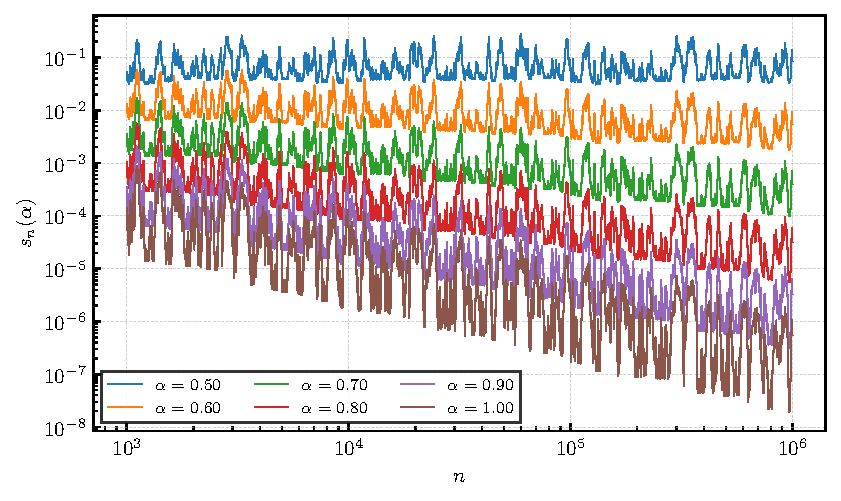
\includegraphics[width=0.9\textwidth]{fig_sn.pdf}
\caption{The M\"obius error $s_n(\alpha)$ for $\alpha = 0.50, 0.60, \dots, 1.00$ and
$10^3 \leq n \leq 10^6$, in log--log scale.}
\label{fig:sn}
\end{figure}

\begin{table}[htb!]
\centering
\footnotesize
\begin{tabular}{|c|cc|cc|cc|}
\hline
\multirow{2}{*}{$\alpha$} & \multicolumn{2}{c|}{$10^{3} \leq n < 10^{4}$} & \multicolumn{2}{c|}{$10^{4} \leq n < 10^{5}$} & \multicolumn{2}{c|}{$10^{5} \leq n \leq 10^{6}$} \\
\cline{2-7}
 & $\max s_n$ & $\min s_n$ & $\max s_n$ & $\min s_n$ & $\max s_n$ & $\min s_n$ \\
\hline\hline
0.50 & $2.617\mathrm{e}{-1}$ & $3.181\mathrm{e}{-2}$ & $2.772\mathrm{e}{-1}$ & $3.408\mathrm{e}{-2}$ & $2.530\mathrm{e}{-1}$ & $3.079\mathrm{e}{-2}$ \\
0.55 & $1.219\mathrm{e}{-1}$ & $1.189\mathrm{e}{-2}$ & $9.722\mathrm{e}{-2}$ & $1.086\mathrm{e}{-2}$ & $7.554\mathrm{e}{-2}$ & $7.605\mathrm{e}{-3}$ \\
0.60 & $5.866\mathrm{e}{-2}$ & $4.390\mathrm{e}{-3}$ & $3.954\mathrm{e}{-2}$ & $3.213\mathrm{e}{-3}$ & $2.298\mathrm{e}{-2}$ & $1.776\mathrm{e}{-3}$ \\
0.65 & $3.162\mathrm{e}{-2}$ & $1.632\mathrm{e}{-3}$ & $1.683\mathrm{e}{-2}$ & $9.559\mathrm{e}{-4}$ & $7.140\mathrm{e}{-3}$ & $4.171\mathrm{e}{-4}$ \\
0.70 & $1.740\mathrm{e}{-2}$ & $6.106\mathrm{e}{-4}$ & $7.338\mathrm{e}{-3}$ & $2.857\mathrm{e}{-4}$ & $2.393\mathrm{e}{-3}$ & $9.806\mathrm{e}{-5}$ \\
0.75 & $9.798\mathrm{e}{-3}$ & $2.296\mathrm{e}{-4}$ & $3.291\mathrm{e}{-3}$ & $8.578\mathrm{e}{-5}$ & $8.578\mathrm{e}{-4}$ & $2.316\mathrm{e}{-5}$ \\
0.80 & $5.662\mathrm{e}{-3}$ & $8.677\mathrm{e}{-5}$ & $1.528\mathrm{e}{-3}$ & $2.584\mathrm{e}{-5}$ & $3.197\mathrm{e}{-4}$ & $5.499\mathrm{e}{-6}$ \\
0.85 & $3.370\mathrm{e}{-3}$ & $3.293\mathrm{e}{-5}$ & $7.396\mathrm{e}{-4}$ & $7.811\mathrm{e}{-6}$ & $1.254\mathrm{e}{-4}$ & $1.313\mathrm{e}{-6}$ \\
0.90 & $2.073\mathrm{e}{-3}$ & $1.255\mathrm{e}{-5}$ & $3.768\mathrm{e}{-4}$ & $2.368\mathrm{e}{-6}$ & $5.263\mathrm{e}{-5}$ & $3.157\mathrm{e}{-7}$ \\
0.95 & $1.323\mathrm{e}{-3}$ & $4.793\mathrm{e}{-6}$ & $2.039\mathrm{e}{-4}$ & $7.196\mathrm{e}{-7}$ & $2.405\mathrm{e}{-5}$ & $7.693\mathrm{e}{-8}$ \\
1.00 & $8.784\mathrm{e}{-4}$ & $1.838\mathrm{e}{-6}$ & $1.181\mathrm{e}{-4}$ & $2.192\mathrm{e}{-7}$ & $1.217\mathrm{e}{-5}$ & $1.926\mathrm{e}{-8}$ \\
\hline
\end{tabular}
\caption{Largest and smallest values of the M\"obius error $s_n(\alpha)$ over
each decade of $n$, for $\alpha = 0.50, 0.55, \dots, 1.00$, computed at $3001$
logarithmically spaced values of $n \in [10^3, 10^6]$.}
\label{tab:envelope}
\end{table}

On the critical line the M\"obius error does not decay: over the three decades the
maxima of $s_n(1/2)$ are $0.262$, $0.277$ and $0.253$, and the minima
$3.18 \cdot 10^{-2}$, $3.41 \cdot 10^{-2}$ and $3.08 \cdot 10^{-2}$. This is the
behaviour forced by the result of B\'aez-Duarte~\cite{baez-unitary}, by which
$s_n(1/2) \not\to 0$. For every $\alpha > 1/2$, on the other hand, both the maxima and
the minima decrease geometrically from one decade to the next, and
Figure~\ref{fig:exponent} shows that the rate is very close to $10^{1-2\alpha}$ per
decade: over the whole range the observed changes of $\log_{10}$ per decade differ from
$1 - 2\alpha$ by less than $0.08$. The data are thus consistent with
\[
s_n(\alpha) \asymp n^{1-2\alpha}, \qquad \tfrac12 \leq \alpha \leq 1,
\]
for the envelope of the oscillations, and in particular with $s_n(\alpha) \to 0$ for
every $\alpha > 1/2$. The convergence is very slow near the critical line: for
$\alpha = 0.55$ the error decreases only by a factor $10^{0.1} \approx 1.26$ per decade,
so that for moderate $n$ the behaviour for $\alpha$ slightly above $1/2$ is hard to tell
apart from that on the critical line. The exponent $1 - 2\alpha$ is precisely the one
given by the lower bound~\eqref{eq:lowerM1} when $M_1(n)$ is of order $n^{-1/2}$, and
the largest peaks of $s_n(\alpha)$ in Figure~\ref{fig:sn} occur where $n M_1(n)^2$ is
large.

\begin{figure}[htb!]
\centering
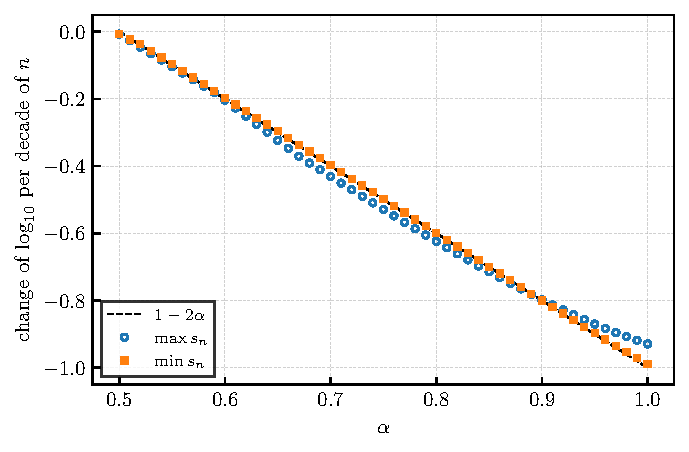
\includegraphics[width=0.7\textwidth]{fig_exponent.pdf}
\caption{Change of $\log_{10} \max s_n(\alpha)$ and of $\log_{10} \min s_n(\alpha)$ per
decade of $n$, from $10^3 \leq n < 10^4$ to $10^5 \leq n \leq 10^6$, for
$\alpha = 0.50, 0.51, \dots, 1.00$, compared with $1 - 2\alpha$ (dashed).}
\label{fig:exponent}
\end{figure}

These observations must be read with care. By Proposition~\ref{main-prop}, a proof that
$s_n(\alpha) \to 0$ for some $\alpha < 1$ would give a zero-free half-plane
$\mathbb{C}_\alpha$, far beyond the known zero-free regions of $\zeta$. The behaviour
observed is the one expected under RH, under which $M_1(n) = O(n^{-1/2+\varepsilon})$,
but no finite computation can rule out the alternative: by Theorem~\ref{thm:lower}, a
zero $\rho$ with $\mathrm{Re}\,\rho > \alpha$ only forces
$s_n(\alpha) \geq 2(\mathrm{Re}\,\rho - \alpha)/|\rho|^2$, and since every zero with
$|\mathrm{Im}\,\rho| \leq 3 \cdot 10^{12}$ lies on the critical line~\cite{platt}, this
floor would be smaller than $10^{-24}$.

\subsection{The optimal error on the critical line}\label{subsec:dn}

The critical line is the one place in the range studied where $S_n$ demonstrably
fails: by B\'aez-Duarte~\cite{baez-unitary} the Möbius coefficients do not sum to
$E$ at $\alpha = 1/2$, and the undamped oscillations of Figure~\ref{fig:sn}
are the price of this fixed choice. Since it is exactly at $\alpha = 1/2$ that
Theorem~\ref{thm:bagchi} formulates the RH, the natural question is what this
failure rules out. The answer is: nothing about the subspaces
$\mathrm{span}\{G_2, \dots, G_n\}$ themselves, since $\mu(k)$ is only one
admissible choice of coefficients, and it is the subspaces, not the choice, that
Theorem~\ref{thm:lower} ties to the zeros of $\zeta$. This is what motivates the
present experiment: we replace $s_n(1/2)$ by the optimal error $d_n(1/2)^2$ of
Subsection~\ref{subsec:lower}, the true distance from $E$ to
$\mathrm{span}\{G_2, \dots, G_n\}$ on the critical line, which removes the
coefficients from the picture by optimising over all of them. It is computed by
the Gram matrix method of Subsection~\ref{subsec:method}.

Figure~\ref{fig:dn} contrasts the two sequences, and Table~\ref{tab:dn} records
their values at selected $n$. While the Möbius error $s_n(1/2)$ remains near
$10^{-1.5}$ with persistent oscillations, the optimal error $d_n^2$ decreases
steadily, though very slowly, and satisfies $d_n^2 \leq s_n(1/2)$ throughout the
computed range. The ``divergence'' on the critical line is therefore a statement
about the coefficients rather than about the subspaces: the obstruction lies in the
fixed choice $c_k = \mu(k)$, while the true distance from $E$ to
$\mathrm{span}\{G_2, \dots, G_n\}$ continues to decrease over the range accessible
to stable computation.

\begin{figure}[htb!]
\centering
% The graphic is saved first so that the table can be centred inside a box of
% exactly the same height; the two captions then start on the same line.
\sbox{\dnbox}{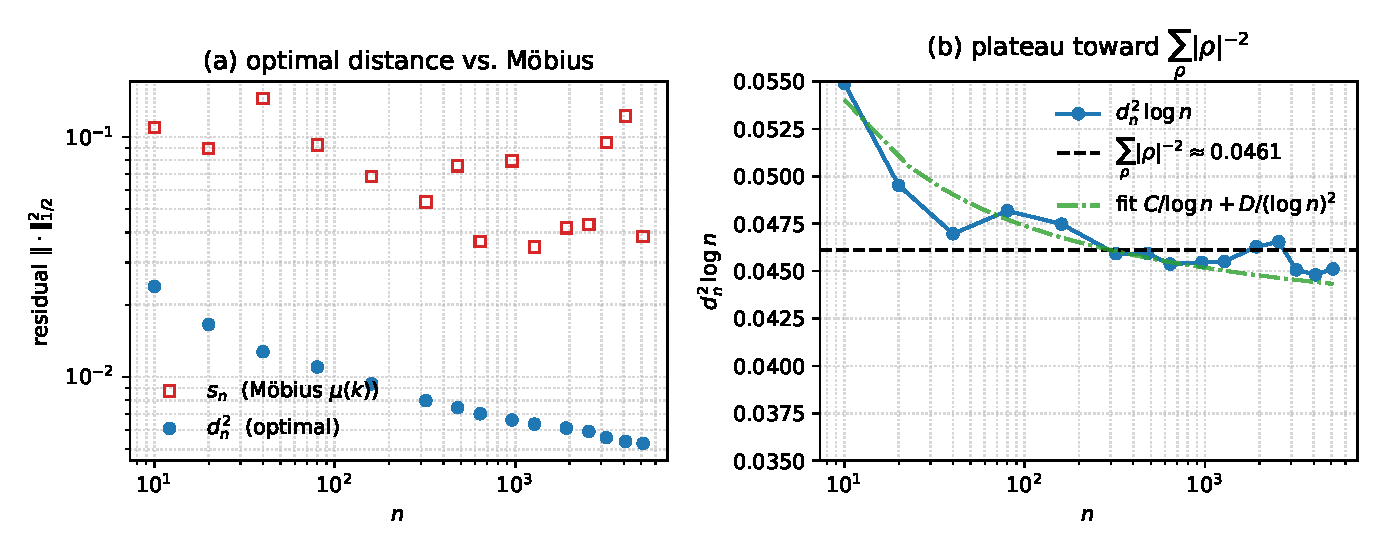
\includegraphics[width=0.52\textwidth,viewport=0 0 331 267,clip]{fig_dn.pdf}}
\begin{minipage}[t]{0.52\textwidth}
\centering
\vspace{0pt}
\usebox{\dnbox}
\caption{The optimal error $d_n(1/2)^2$ (blue) and the Möbius error
$s_n(1/2)$ (red) on the critical line, $2 \leq n \leq 5120$, in log--log scale.}
\label{fig:dn}
\end{minipage}\hfill
\begin{minipage}[t]{0.44\textwidth}
\centering
\vspace{0pt}
\sbox{\dntab}{\renewcommand{\arraystretch}{1.2}%
\begin{tabular}{|r|c|c|}
\hline
$n$ & $d_n(1/2)^2$ & $s_n(1/2)$ \\
\hline
\hline
$40$   & $1.273\mathrm{e}{-2}$ & $1.442\mathrm{e}{-1}$ \\
$160$  & $9.355\mathrm{e}{-3}$ & $6.846\mathrm{e}{-2}$ \\
$640$  & $7.022\mathrm{e}{-3}$ & $3.657\mathrm{e}{-2}$ \\
$1280$ & $6.361\mathrm{e}{-3}$ & $3.473\mathrm{e}{-2}$ \\
$2560$ & $5.931\mathrm{e}{-3}$ & $4.312\mathrm{e}{-2}$ \\
$5120$ & $5.282\mathrm{e}{-3}$ & $3.850\mathrm{e}{-2}$ \\
\hline
\end{tabular}}%
% Pad by exactly the slack, so the table drops to the foot of the panel
% while the panel keeps the height of the graphic and the captions stay level.
\parbox[c][\dimexpr\ht\dnbox+\dp\dnbox\relax][c]{\linewidth}{\centering
\vspace*{\dimexpr\ht\dnbox+\dp\dnbox-\ht\dntab-\dp\dntab-\baselineskip\relax}
\usebox{\dntab}}
\captionof{table}{The same two errors at selected $n$; in every case
$d_n^2 \leq s_n(1/2)$.}
\label{tab:dn}
\end{minipage}
\end{figure}

% \subsection{Concluding discussion}\label{subsec:discussion}

% The three experiments are consistent: the cost of approximating $E$ by $S_n$
% grows sharply, with a tolerance-dependent transition, as $\alpha \to 1/2$
% (Subsection~\ref{subsec:tol}); near $\alpha = 1$, $s_n(\alpha)$ decays steadily,
% supporting the persistence of Theorem~\ref{main-teo} into the strip
% (Subsection~\ref{subsec:endpoints}); and on the critical line, the failure of
% $S_n$ is attributable to the Möbius coefficients rather than the subspaces,
% since $d_n(1/2)^2$ continues to decrease (Subsection~\ref{subsec:dn}).

% We stress, finally, the conditional nature of this reading. By
% Proposition~\ref{main-prop}, genuine convergence $S_n \to E$ for some
% $1/2 \leq \alpha < 1$ would place $E$ in the closed span of
% $\{G_k : k \geq 2\}$ and hence furnish a zero-free half-plane
% $\mathbb{C}_\alpha$ deep within the critical strip, a conclusion lying far
% beyond all currently known zero-free regions and widely regarded as being as
% difficult as the Riemann Hypothesis itself. The evidence presented here is
% therefore numerical and suggestive, not a proof.

\begin{thebibliography}{99}
    \bibitem{apostol}
    T. M. Apostol, Introduction to analytic number theory. UTM Springer, 1976.
	
	\bibitem{baez}
	L. Báez-Duarte, A strengthening of the Nyman-Beurling criterion for the Riemann hypothesis, Atti Acad. Naz. Lincei 14 (2003) 5-11.

    % \bibitem{BD_Arithmetical}

    % L, Baez-Duarte. Arithmetical Aspects of Beurling's Real Variable Reformulation of the Riemann Hypothesis. arXiv preprint math/0011254 (2000).
   \bibitem{baez-unitary}
  L. Báez-Duarte, A class of invariant unitary operators, Adv. Math., 144, No. 1 (1999), 1-12.

    \bibitem{Balazard}
    M. Balazard and E. Saias. Notes sur la fonction $\zeta$ de Riemann, 1. Adv. Math., Vol. 139 (1998) 310–321.
    
	
	\bibitem{bagchi}
	B. Bagchi, On Nyman, Beurling and Báez-Duarte's Hilbert space reformulation of the Riemann hypothesis, Proc. Indian Acad. Sci. Math. Sci. 116 (2) (2006) 137-146.

    \bibitem{beurling}
    A. Beurling, A closed problem related to the Riemann zeta-function. Proc. Nat. Acad. Sci., 41(5), 312-314, 1955.

    \bibitem{noor-charles}
    A. Ghosh, K. Kremnitzer, W. Noor, C. F. Santos, Zero-free half-planes of the $\zeta$-function via spaces of analytic functions, Adv. Math. 455 (2024) 109872.
	
	\bibitem{2}
	H. Hedenmalm, P. Lindqvist, K. Seip, A Hilbert space of Dirichlet series and systems of dilated functions in $L^{2}(0,1)$, Duke Math. J. 86 (1997) 1-37. MR 99i:42033.

    \bibitem{manzur-noor-santos}
    J. Manzur, S. W. Noor, and C. F. Santos. A weighted composition semigroup related to three open problems. J. Math. Anal. Appl. 525 (2023) 127261.
	
	
	%\bibitem{3}
	%N. Nikolski, In a shadow of the RH: cyclic vectors of the Hardy spaces on the Hilbert multidisc, Ann. Inst. Fourier 62 (5) (2012) 1601-1626.
	
	\bibitem{waleed1}
	S. W. Noor, A Hardy space analysis of the Báez-Duarte criterion for the RH, Adv. Math. 350 (2019) 242-255.

    \bibitem{Nyman}
      B. Nyman, On some groups and semigroups of translations. Thesis, Uppsala, 1950.

    \bibitem{platt}
    D. Platt and T. Trudgian, The Riemann hypothesis is true up to $3 \cdot 10^{12}$, Bull. London Math. Soc. 53 (2021) 792-797.

    \bibitem{6}
	H. Queffélec, K. Seip, Aproximation numbers of composition operators on the $H^{2}$ space of Dirichlet series, J. Funct. Anal. 268 (2015) 1612-1648.

    \bibitem{rudin}
    W. Rudin, Real and Complex Analysis, 3rd ed., McGraw-Hill, New York, 1987.

    \bibitem{titchmarsh}
    E. C. Titchmarsh, The Theory of the Riemann Zeta-Function, 2nd ed., revised by D. R. Heath-Brown, Oxford University Press, 1986.

      \bibitem{Weingartner}
    A. Weingartner. On a question of Balazard and Saias related to the Riemann hypothesis. Adv. Math. Vol. 208  (2007) 905–908. 
	
	
\end{thebibliography}


\end{document}